\subsection{Assets}

Das Modul Assets bietet einfachen Zugriff auf als .j3o gespeicherte Modelle, indem pro Model ein Assetdeskriptor vorhanden ist, welcher
in Json geschrieben ist und von einem \textit{JsonModelProvider} gelesen und verarbeitet wird. Die Modelle liegen dann als Node vor und können so einfach
in den Scenegraph eingebunden werden. Ausserdem unterstützen \textit{AbstractModelProvider} (also auch \textit{JsonModelProvider}) das asynchrone Laden von Modellen
auf einem separaten Thread und das Updaten eines Ladebildschirms. Ein \textit{JsonModelProvider} lädt immer ein ebenfalls in Json beschriebenes \textit{AssetPack},
welches aus benannten Gruppierungen von Assets besteht.

\begin{figure}[htbp]
    \centering
    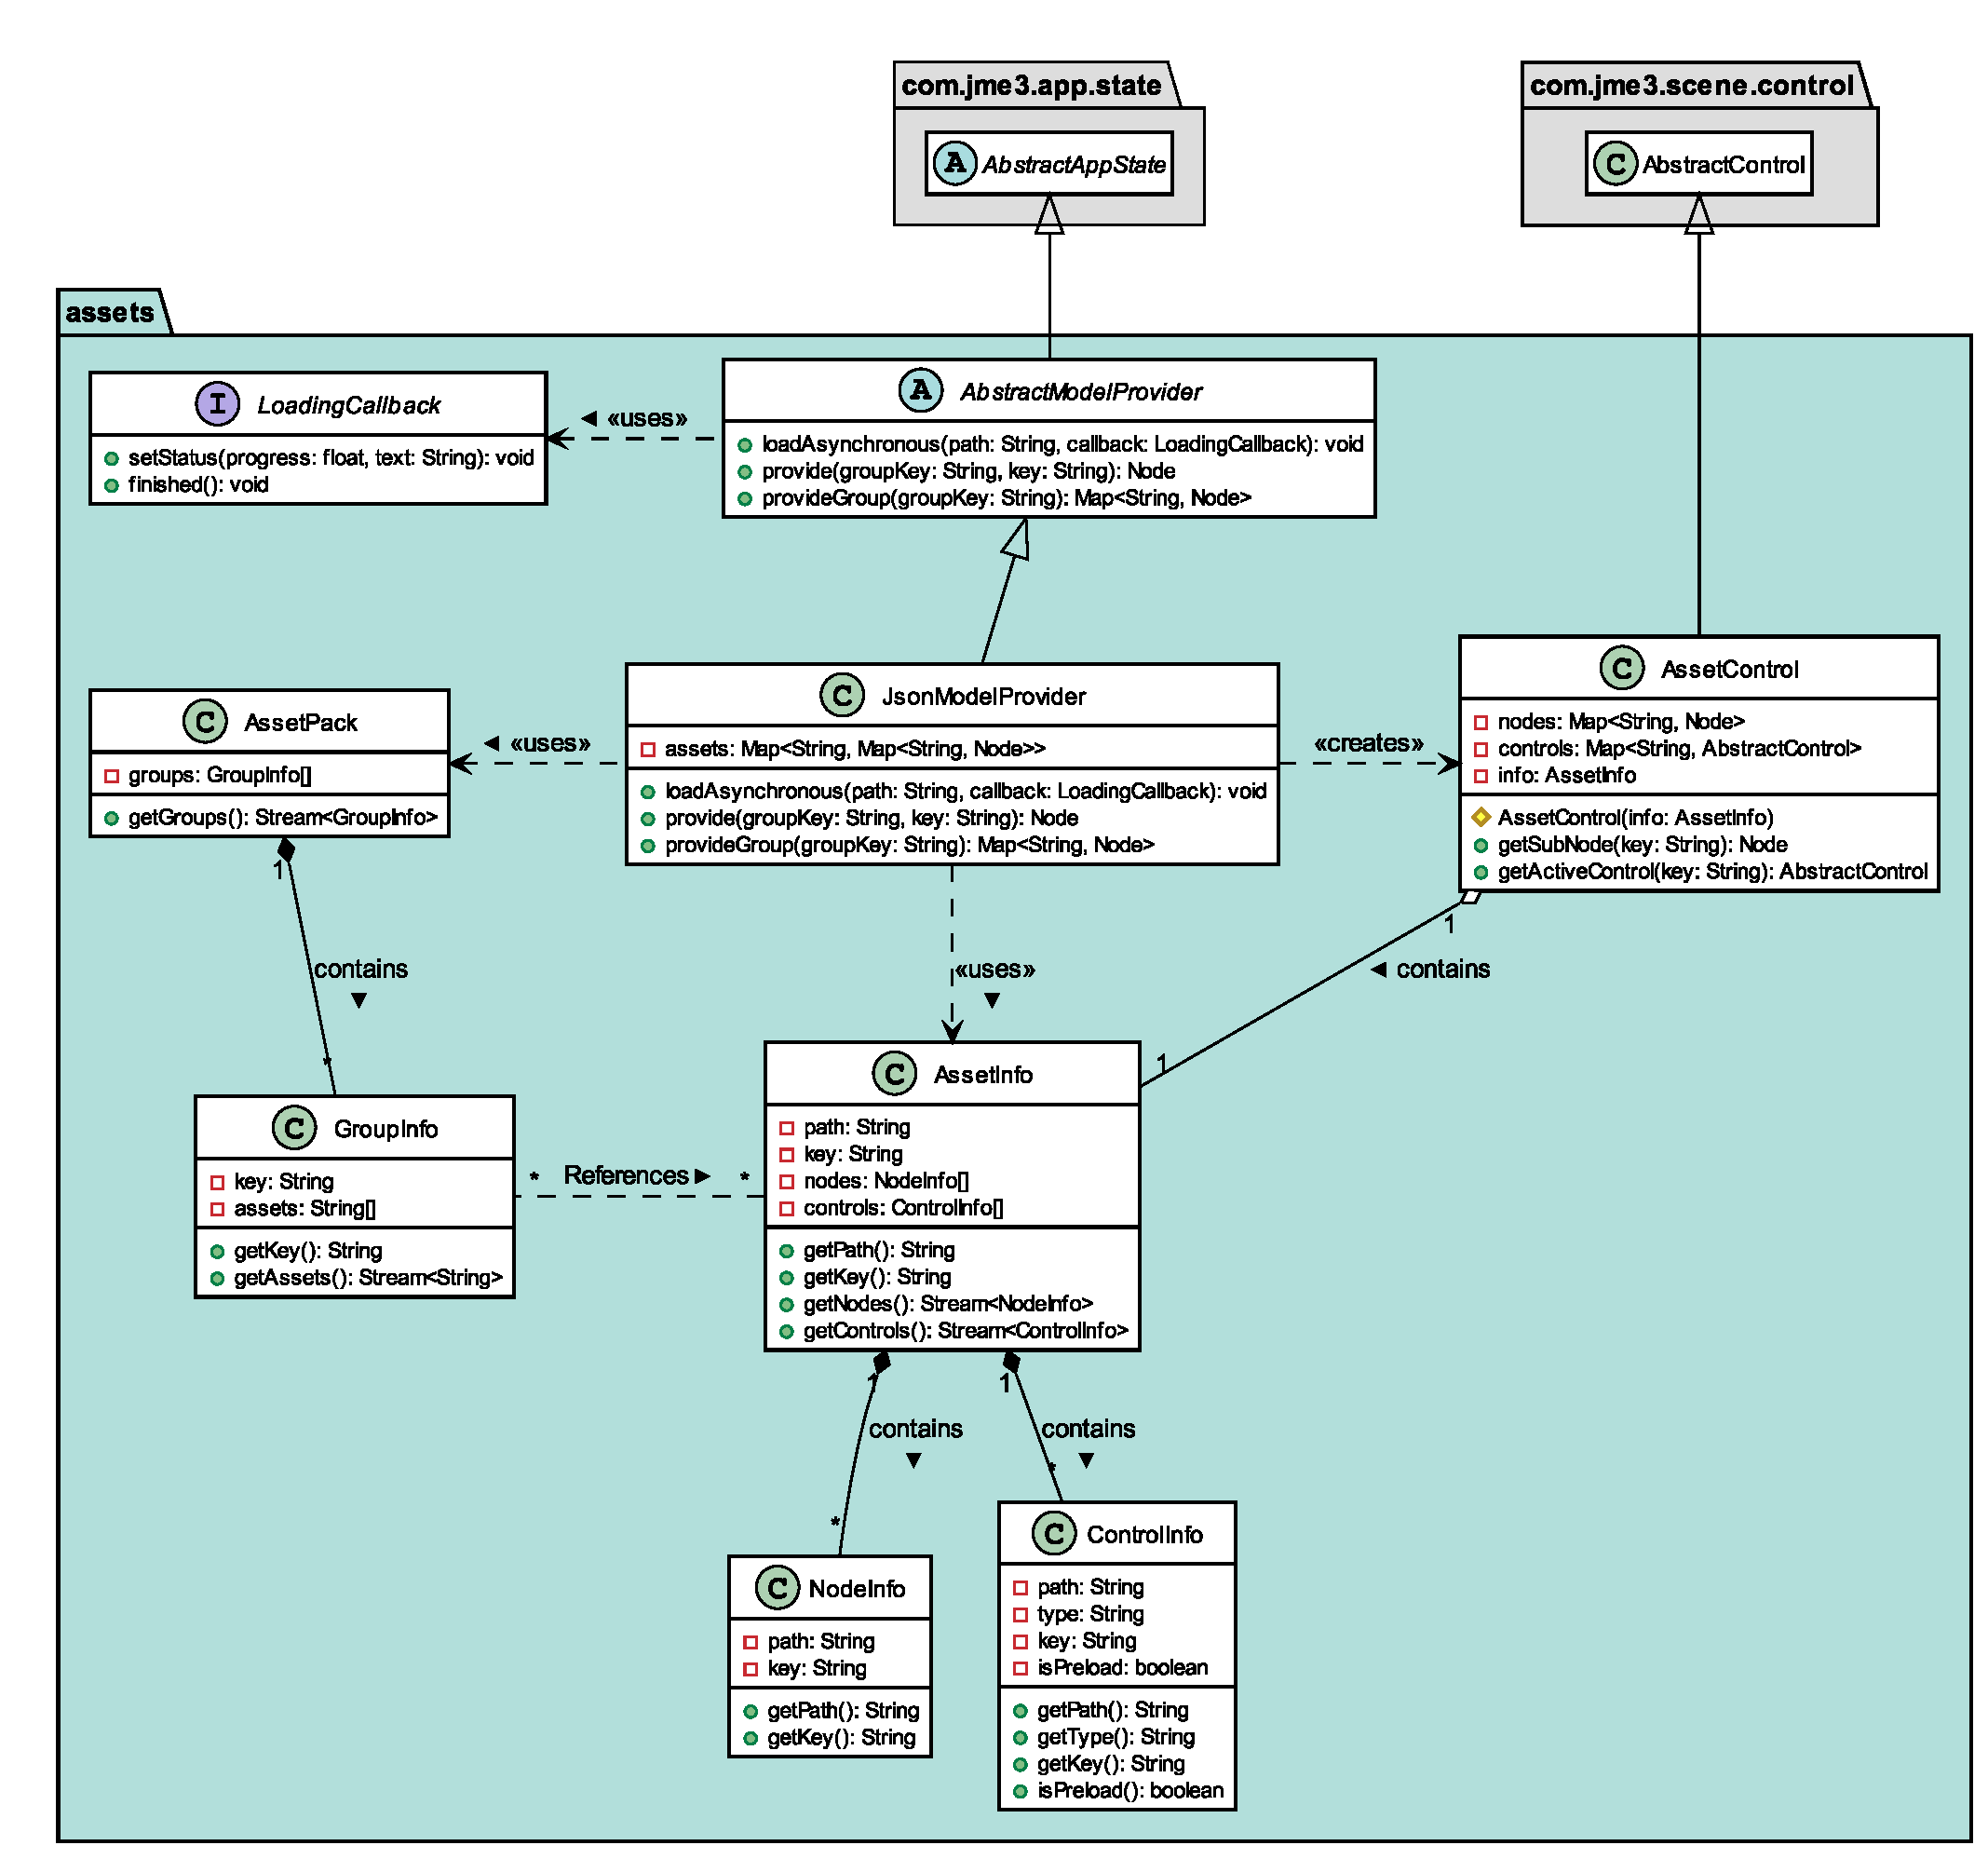
\includegraphics[width=\linewidth]{Assets/assets.eps}
    \caption{Assets Klassen-Diagram}
\end{figure}

\pagebreak